\documentclass[11pt]{article}
\usepackage{ucs}
\usepackage[utf8x]{inputenc}
\usepackage{geometry}
\usepackage[greek,english]{babel}
\newcommand{\en}{\selectlanguage{english}}
\newcommand{\gr}{\selectlanguage{greek}}
\usepackage{amsmath}
\usepackage{amssymb}
\usepackage{mathtools}
\usepackage{float}
\usepackage{graphicx}
%\usepackage{fullpage}
\usepackage{tikz}
\usepackage{titlesec}
\usepackage{caption}
\setcounter{secnumdepth}{4}
\usepackage[bottom]{footmisc}
\usepackage{a4wide}
\usepackage{xcolor} % colors
\usepackage[toc,page]{appendix} % for appendices
\usepackage{csquotes} % for quotes
\usepackage{cancel} % for canceling values to zero

\allowdisplaybreaks % allows split between pages

\DeclarePairedDelimiter{\ceil}{\lceil}{\rceil}
\DeclarePairedDelimiter\floor{\lfloor}{\rfloor}
\usepackage{wrapfig} % wrap text to figure


\usepackage{fancyhdr} % for header
%\pagestyle{fancy}
%\fancyhf{}
%\fancyfoot[C]{\thepage} % centere number of page
%\fancyhead[R]{\rightmark}
\usepackage{bm} % BOLD

\usepackage{listings}

\usepackage{caption}
\usepackage{subcaption}
\usepackage{algorithmic} % for algorithms


\newcommand{\approxtext}[1]{\ensuremath{\stackrel{\text{#1}}{\approx}}}

\renewcommand{\footrulewidth}{0.4pt}% default is 0pt

\usepackage[framed]{matlab-prettifier}


\newcommand\numberthis{\addtocounter{equation}{1}\tag{\theequation}}
\renewcommand{\lstlistingname}{Code}


\DeclareMathOperator*{\argmax}{argmax} % FOR ARGMAX
\DeclareMathOperator*{\argmin}{argmin} % FOR ARGMIN


\begin{document}
	\pagenumbering{gobble} 

	\begin{titlepage}
		\title{
			{\Huge \textbf{Autonomous Agents}} \\
		\vspace{10mm}
		{\Large {Bayesian Classification
	}}} 
		\author{\gr Παπαγεωργίου Βασίλειος (ΑΜ: 2016030080) \en}
		\date{\textit{\today}}
		\maketitle
		\newpage
		\tableofcontents
		\newpage
	\end{titlepage}
	\pagenumbering{arabic}
	
	\section{Introduction}
	In this project we study the case of a specific type of classifiers, called \textbf{Bayesian Classifiers}, a specific type of classifiers which make use of the Bayes theorem to assign labels to data, aiming to maximize the posterior probability. The aforementioned method was tested in the widely known and used \textbf{alarm network} as well as in a \textbf{medical network} which models the dependencies between causes and symptoms for a variety of breathing diseases. The outline of the report is as follows: In [\ref{sec:bayesian_networks}] we describe the fundamentals of bayesian networks. In [\ref{sec:bayesian_classifiers}] we set the basic framework of statistical learning and the general philosophy behind bayesian classifiers, in [\ref{sec:learning_bayesian_networks}] we describe the process of utilizing bayesian networks for statistical learning using two specific black approaches and lastly in [\ref{sec:experiments}] we describe the proposed implementations and the simulation results.
	
	\section{Bayesian Networks \label{sec:bayesian_networks}}
	Bayesian Networks (BN) is a specific graphical model that is used to manipulate joint distributions of random variables, managing to efficiently model their dependencies, in a systematic way. More specifically, it consists of a directed and acyclic graph (DAG) whose nodes are random variables; each random variable $X_i$ has a conditional distribution $\text{Pr}(X_i | \text{parents}(X_i))$ which is \textbf{only dependent on its parents in the graph} and is stored in a table called \textbf{Conditional Probability Table} (CPT). As a result, we can write:
	
	\begin{align*}
		\text{Pr}(x_1,\dots,x_n) = \prod_{i=1}^{n}\text{Pr}(x_i |  \text{parents}(X_i))
	\end{align*}
	
	The most basic task for any probabilistic inference system - and as a result for BN's- is to calculate the posterior probability distribution for a set of query variables, given the observations of a set of evidence variables. This is called \textbf{exact inference} and there are various algorithms who calculate the answers in such queries. What we implement in this project is an algorithm called \textbf{variable enumeration}. This algorithm is based on the simple observation that any query $\text{Pr}(X|\mathbf{e})$ can be answered by:
	
	\begin{align*}
		\text{Pr}(X|\mathbf{e}) = a\text{Pr}(X,\mathbf{e}) = a\sum_{\mathbf{y}}\text{Pr}(X,\mathbf{e},\mathbf{y})
	\end{align*}
	where $a$ is a normalization constant, $\mathbf{e}$ the set of evidence variables and $\mathbf{y}$ the set of hidden variables.
	\par
	For the purpose of generating artificial datasets, we also utilize an algorithm that approximately answers queries such the one that was described above, which belongs to the set of randomized \textbf{Monte Carlo} sampling algorithms, and is called \textbf{prior sampling}. What this algorithm suggests is that each variable is sampled according to the conditional distribution given the values of its already sampled parents.
	\section{Bayesian Classifiers \label{sec:bayesian_classifiers}}	
	A statistical \textbf{classifier} is a function $f:\Omega_\mathbf{X} \rightarrow \Omega_C$ that maps the values of attributes $\mathbf{X} \in \mathbb{R}^n$ to a unique class label $c \in \Omega_C = \{c_1,\dots,c_m\}$. In order to induce such a function, a dataset $\mathcal{D}$ with $N$ labeled tuples $<\mathbf{X}, C>$ is required, to which a variety of algorithms can be applied aiming to learn the function $f$ that best describes the data in $\mathcal{D}$ and generalizes well in the case of unseen data. The goal is to find a function $f$ that when given an observation $\mathbf{x}$, it assigns $c^*$ to it, where:
	
	\begin{align*}
		c^* = \argmax_j\{\text{Pr}(c_j|\mathbf{x})\} \numberthis \label{eq:class}
	\end{align*}
	Bayesian classifiers are a specific case of statistical classifiers, as were described above. The term "Bayesian" stems from the fact that we use \textbf{Bayes' theorem} in (\ref{eq:class}) getting:
	
	\begin{align*}
		c^* = \argmax_j\{\text{Pr}(c_j)\text{Pr}(\mathbf{x}|c_j)\} \numberthis \label{eq:class2}
	\end{align*}
	Usually, the space of $\mathbf{x}$ is of a fairly high dimension, which leads to the fact that the calculation of the term $\text{Pr}(\mathbf{x}|c_j)$ in (\ref{eq:class2}) is challenging. Hence, it is necessary to make some independence assumptions in order to lower the complexity of the system, which are described later in the report.
	
	\subsection{Learning Bayesian Networks \label{sec:learning_bayesian_networks}}
	The Bayesian Networks' learning, consists of two phases, one to learn the structure of the DAG of attributes and one to estimate the parameters of the conditional distributions (the values of CPT's) using a specific approach (in our case \textbf{maximum likelihood}). More formally, given a set of random variables $\mathbf{X} = \{X_1, X_2,\dots,X_n\}$ and a training dataset $\mathcal{D} = \{\mathbf{x}_1,\dots,\mathbf{x}_N\}$ our goal is to induce a BN that best matches $\mathcal{D}$.
	
	\subsubsection{Naive Bayes \label{naive_bayes}}
	Naive Bayes classifier makes the "naive" assumption that all the attributes are conditionally independent, given the value of the label. As a result, it holds that:
	\begin{align*}
		\text{Pr}(\mathbf{x}|c) = \prod_{i} \text{Pr}(X_i=x_i|c)
	\end{align*}
	Hence, we can rewrite (\ref{eq:class2}) as:
	\begin{align*}
		c^* = \argmax_j\{\text{Pr}(c_j) \prod_{i}\text{Pr}(X_i=x_i|c_j)\}
	\end{align*}
	If we see this classifier as a BN, its topology is similar to the one represented in Figure \ref{fig:naive_bayes_net}, where the label is the only parental vertex of each variable, implying that all variables are conditionally independent given the label.
	\begin{figure}[H]
		\makebox[\textwidth][c]{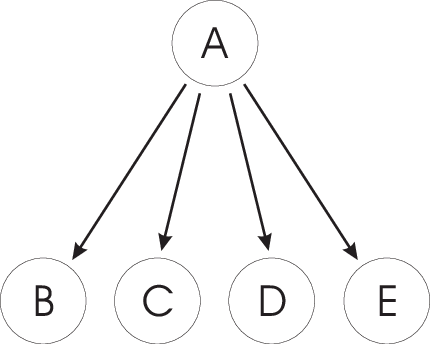
\includegraphics[width=.35\textwidth]{figs/naive_bayes_net.png}}
		\caption{Naive Bayes classifier BN structure example.}
		\label{fig:naive_bayes_net}
	\end{figure}
	
	\subsubsection{Tree Augmented Naive Bayes \label{sec:tan_naive_bayes}}
	Tree Augmented Naive (TAN) Bayes classifiers loosen the tight restriction of conditional independence of all the attributes of the problem, by allowing to each variable to have at most one other parent other than the label in the network. The network of such a classifier can be seen in Figure \ref{fig:tan_net}.
	
	\begin{figure}[H]
		\makebox[\textwidth][c]{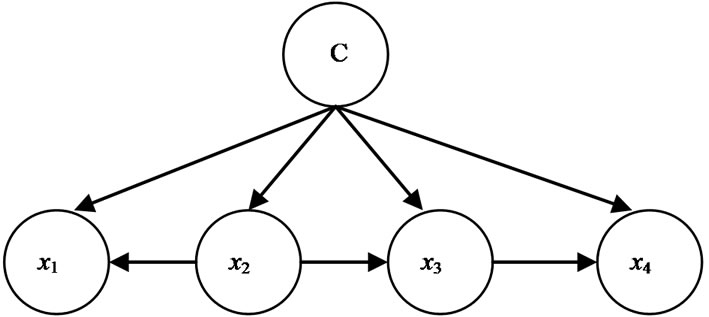
\includegraphics[width=.5\textwidth]{figs/tan_net.jpg}}
		\caption{Tree Augmented Naive Bayes classifier BN structure example.}
		\label{fig:tan_net}
	\end{figure}
	We can see that in contrary to the case of Naive Bayes classifier, the structure of the network is not know. As a result, we have to utilize an algorithm that is used for the task of learning bayesian networks' structures. The algorithm that we use is the \textbf{Chow Liu} algorithm, which is able to induce BN's topology when the number of parents of each node is restricted, while its goal being to find a \textbf{tree that maximizes the likelihood of the training data}.
	\par
	First of all, we have to highlight that the \textbf{mutual information} of two random variables is given by:
	\begin{align*}
		I(X,Y) = \sum_{x,y}p_{XY}(x,y)\log\dfrac{p_{XY}(x,y)}{p_X(x)P_Y(y)}
	\end{align*}
	What Chow Liu suggests is to firstly calculate the weight $I(X_i, X_j)$, $\forall i \neq j$, find a \textbf{maximum} weight spanning tree from the initially fully connected graph and make the graph directed starting from a random vertex using a traversal like BFS or DFS.
	\par
	TAN classifiers make use of this algorithm to induce the dependency relationships between the different attributes but the label. More specifically, Chow Liu is initially used to all the attributes except for the label, using the conditional mutual information of the variables given the label as the weight. After that, the label is added as a parental vertex to each variable of the graph and the CPT's are calculated from the training data (in our case using \textbf{maximum likelihood} estimation).
	\section{Implementation \label{sec:experiments}}
	\subsection{Code}
	The aforementioned techniques and algorithms were implemented using raw Python. The code structure is as follows:
	\begin{itemize}
		\item \textbf{main.py}: contains the driver code that is used to perform the experiments
		\item \textbf{graph\_utils.py}: contains the implementation of various graph operations (topological sort, prim's algorithm) 
		\item \textbf{bn\_utils.py}: contains the implementation of a class named \textbf{BayesianNetwork} through which the representation as well as the \textbf{varibale enumeration} algorithm are implemented.
		\item \textbf{bn\_classifier.py}: contains the implementation of the class \textbf{TANClassifier} through which we implement the TAN as well as the Naive Bayes classifiers.
		\item \textbf{bn\_test.py}: contains code that calculates the classification error of a learnt network.
	\end{itemize}
	\subsection{Experiments}
	The use cases that we use to test the implementation of the algorithms that were described above are the widely know \textbf{alarm} bayesian network that we also saw during the lectures as well as a \textbf{medical} bayesian network used to classify patients based on their symptoms. The topologies of the graphs of the two networks are in Figures \ref{fig:alarm} and \ref{fig:medical_net} respectively.
	
	\begin{figure}[H]
		\makebox[\textwidth][c]{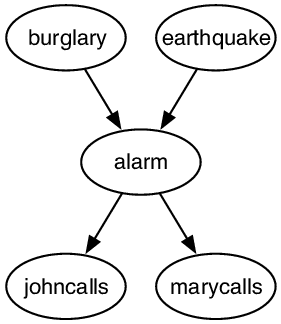
\includegraphics[width=.3\textwidth]{figs/alarm_network.png}}
		\caption{Alarm network.}
		\label{fig:alarm}
	\end{figure}
	\begin{figure}[H]
		\makebox[\textwidth][c]{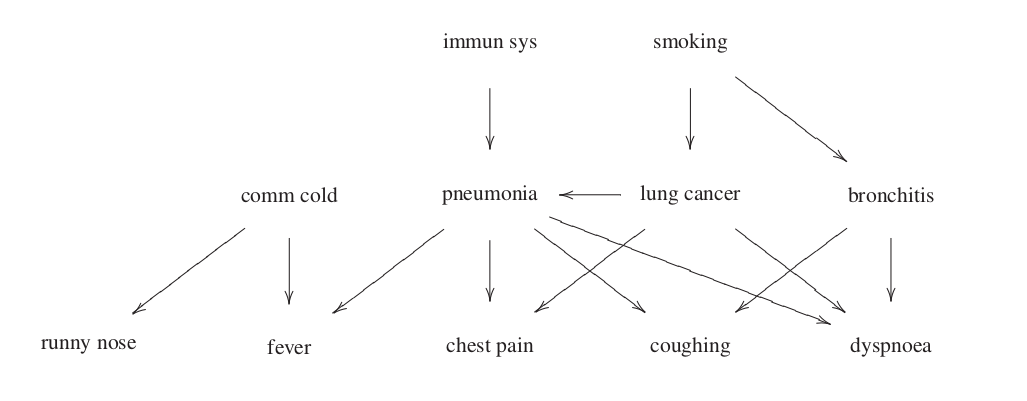
\includegraphics[width=1\textwidth]{figs/medical_network.png}}
		\caption{Medical network.}
		\label{fig:medical_net}
	\end{figure}
	From these two networks, we make use of the prior sampling algorithm to generate two artificial datasets which are afterwards used to build a TAN and a Naive Bayes classifier. We then calculate the mean error percentage of misclassified samples in both cases, having a different label each time. The results are in Figures \ref{fig:error_alarm} and \ref{fig:error_medical} alongside with the misclassification percentage that is yield by the initial networks.
	\par
	We can see that in the case of the alarm network, both TAN and NB classifiers achieve to induce networks that model the random variables' dependencies well for every possible label case. As a result, the misclassification error is only slightly higher compared to using the actual BN, only in some cases.
	\par
	Same conclusions can also be drawn from the case of the medical network. More specifically, both TAN and Naive Bayes reasoning is fairly close to the actual BN, with the Naive Bayes having difficulties to model random variables' relationships - and as a result has a higher error percentage-  in the case where the label is lung\_cancer.
	\begin{figure}[H]
		\makebox[\textwidth][c]{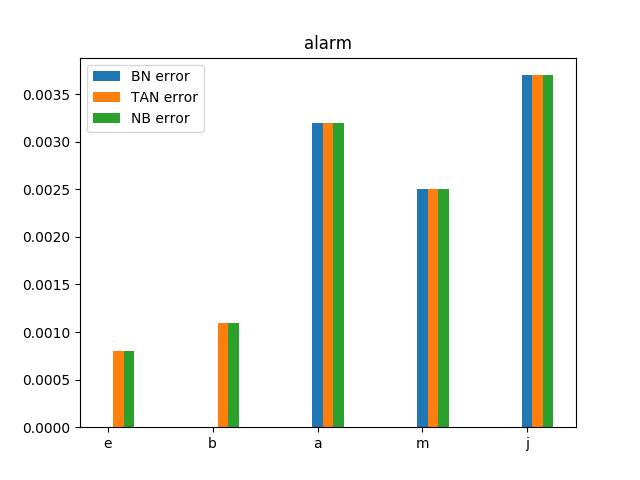
\includegraphics[width=.8\textwidth]{../plots/error_alarm.png}}
		\caption{Alarm network error comparison.}
		\label{fig:error_alarm}
	\end{figure}
	\begin{figure}[H]
		\makebox[\textwidth][c]{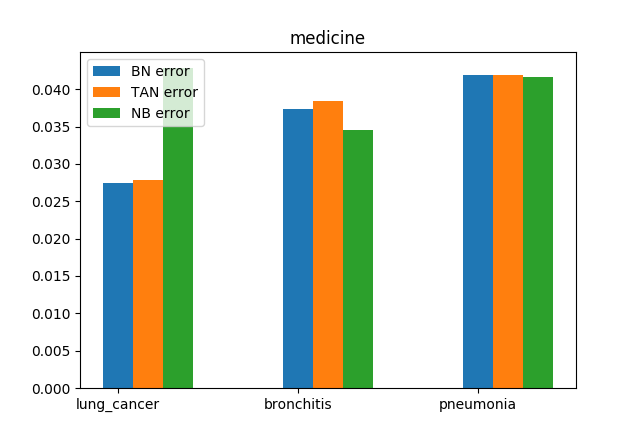
\includegraphics[width=.8\textwidth]{../plots/error_medicine.png}}
		\caption{Medical network error comparison.}
	\label{fig:error_medical}
\end{figure}
\end{document}